\chapter{Revisão Sistemática da Literatura}
\label{cap:rsl}

Esta seção apresenta a Revisão Sistemática de Literatura, utilizada para selecionar trabalhos
relacionados com a proposta da pesquisa para mapear os que aplicam técnicas de análise de
sentimentos a dados ESG, com o objetivo de identificar as principais abordagens, desafios e
oportunidades.

A importância de uma \gls{RSL} reside em sua capacidade de fornecer uma visão abrangente e
metodologicamente rigorosa sobre um determinado campo de estudo. Seguindo uma metodologia
definida, este trabalho busca responder questões cruciais sobre as técnicas utilizadas na análise de
sentimentos aplicada a dados ESG. Ao fazer isso, espera-se contribuir para um entendimento mais
profundo e abrangente das melhores práticas e das lacunas de pesquisa existentes, promovendo o
avanço do conhecimento e a aplicação eficaz dos critérios ESG.

\section{Protocolo da RSL}
\label{sec:protocolo-rsl}

O objetivo de uma Revisão Sistemática da Literatura (RSL) é identificar, avaliar e discutir
trabalhos relevantes a fim de responder uma ou mais questões de pesquisa e identificar lacunas de
pesquisa. Esse objetivo deve ser alcançado através de uma metodologia bem definida, na qual
pode-se obter resultados menos enviesados \cite{dresch2015}.

\subsection{Metodologia da RSL}
\label{subsec:metodologia-rsl}

No protocolo da RSL, define-se, entre outras coisas, como será conduzida a execução da
revisão. O primeiro passo para a elaboração desse protocolo é a definição do objetivo da pesquisa.
O objetivo desta RSL é identificar abordagens para a análise de sentimentos aplicada a dados
relacionados aos princípios ESG utilizando técnicas de Processamento de Linguagem Natural (NLP).
Na Figura \ref{fig:metodologia-rsl} observa-se a metodologia adotada neste trabalho, baseada em
\citeauthor{dresch2015} \citeyear{dresch2015}.

\begin{figure}[h]
    \centering
    \caption{Metodologia da RSL}
    \label{fig:metodologia-rsl}
    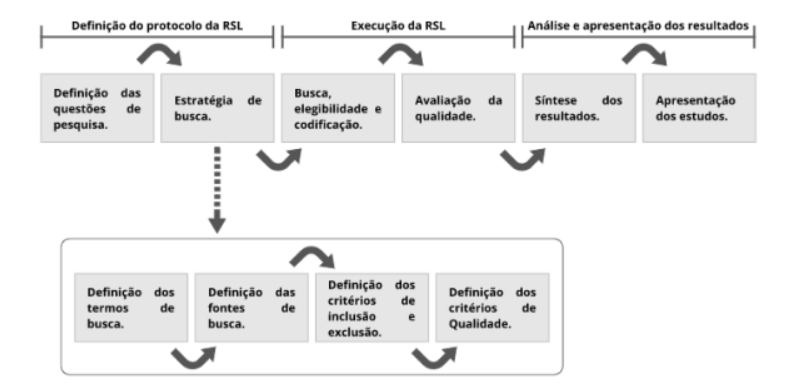
\includegraphics[width=0.85\textwidth]{figuras/metodologia-rsl}
    \legend{Fonte: \citeauthor{lopes2023} \citeyear{lopes2023}.}
\end{figure}

\subsection{Definição das Questões de Pesquisa}
\label{subsec:questoes-rsl}

Após estabelecer o objetivo, o passo seguinte na condução de uma revisão sistemática é
definir as questões de pesquisa que os estudos selecionados devem abordar. Esta etapa é crucial, pois
a habilidade de responder a essas questões é um dos principais critérios para a avaliação dos estudos
primários. Pode-se observar na Tabela \ref{tab:questoes-pesquisa} as questões de pesquisa definidas
para a RSL realizada neste trabalho.

\begin{table}[h]
\caption{Questões de Pesquisa}
\label{tab:questoes-pesquisa}
\begin{tabular}{p{1.5cm}p{11cm}}
\hline
\textbf{ID} & \textbf{Questões de Pesquisa (QP)} \\
\hline
QP1 & Quais técnicas de análise de sentimentos são utilizadas em dados relacionados a ESG? \\
QP2 & O que são indicadores ESG? \\
QP3 & Como a análise de sentimento pode ser utilizada para melhorar o desempenho ESG (\textit{Environmental, Social, and Governance}) de organizações públicas? \\
\hline
\end{tabular}
\legend{Fonte: Autoria Própria (2024).}
\end{table}

\subsection{Estratégia de Busca}
\label{subsec:estrategia-busca}

Após definir as questões de pesquisa, define-se a estratégia de busca dos estudos primários,
especifica-se os termos de busca, as fontes, os critérios de inclusão e exclusão e os critérios de
qualidade.

\subsection{Fontes de Busca}
\label{subsec:fontes-busca}

As fontes de buscas utilizadas para realizar a pesquisa foram:

\begin{alineas}
    \item IEEE Xplore
    \item Capes
    \item Science Direct
\end{alineas}

\subsection{Termos e String de Busca}
\label{subsec:termos-busca}

Para realizar a pesquisa nas fontes de busca selecionadas, os seguintes termos foram
escolhidos para compor a String de busca: ``ESG'', ``sentiment analysis'', ``public perception'' e
``NLP'' que foi inserida depois. Para abranger um maior número de artigos relacionados aos termos,
algumas variações foram adotadas, resultando na seguinte String de busca:

\begin{citacao}
(\textit{``ESG'' AND ``sentiment analysis'' AND ``public perception'' OR ``ESG'' AND ``NLP''}).
\end{citacao}

\subsection{Critérios de Inclusão e Exclusão}
\label{subsec:criterios}

Para filtrar os estudos primários foram definidos critérios de inclusão e exclusão que podem
ser conferidos nas Tabelas \ref{tab:criterios-inclusao} e \ref{tab:criterios-exclusao},
respectivamente.

\begin{table}[h]
\caption{Critérios de Inclusão}
\label{tab:criterios-inclusao}
\begin{tabular}{p{1.5cm}p{11cm}}
\hline
\textbf{ID} & \textbf{Critérios de Inclusão (CI)} \\
\hline
CI1 & Estudos publicados em periódicos (\textit{journals}) \\
CI2 & Estudos com texto completo acessível \\
CI3 & Estudos publicados entre 2020 e 2024 \\
CI4 & Estudos nos quais os termos de busca estejam presentes nos Metadados (título, resumo e palavras-chave) \\
\hline
\end{tabular}
\legend{Fonte: Autoria Própria (2024).}
\end{table}

\begin{table}[h]
\caption{Critérios de Exclusão}
\label{tab:criterios-exclusao}
\begin{tabular}{p{1.5cm}p{11cm}}
\hline
\textbf{ID} & \textbf{Critério de Exclusão (CE)} \\
\hline
CE1 & Estudos fora do objetivo da pesquisa e das questões de pesquisa. \\
\hline
\end{tabular}
\legend{Fonte: Autoria Própria (2024).}
\end{table}

\subsection{Critérios para Avaliação da Qualidade dos Estudos}
\label{subsec:criterios-qualidade}

Para avaliar a qualidade dos estudos incluídos nesta revisão sistemática, foram definidos três
critérios principais. O primeiro critério avalia a qualidade da execução do estudo, focando a precisão
e rigor metodológico. Os dois critérios seguintes avaliam, respectivamente, a adequação do estudo ao
objetivo da pesquisa e a pertinência do estudo ao contexto definido para esta RSL.

Cada estudo foi avaliado de acordo com esses três critérios, sendo classificados como de
qualidade alta, média ou baixa. A partir dessa avaliação, os estudos foram ranqueados globalmente,
seguindo a regra de que: um estudo será considerado de qualidade baixa se apresentar avaliação
baixa em qualquer um dos três critérios; será considerado de qualidade média se tiver pelo menos
um critério avaliado como médio e os demais como altos; e será considerado de qualidade alta se
todos os três critérios forem avaliados como altos. Estes critérios são apresentados na Tabela
\ref{tab:criterios-avaliacao}, adaptada de \citeauthor{lopes2023} \citeyear{lopes2023}.

\begin{table}[h]
\caption{Critérios de Avaliação}
\label{tab:criterios-avaliacao}
\begin{tabular}{p{2cm}p{4.5cm}p{4cm}p{4cm}}
\hline
\textbf{Critério} & \textbf{Qualidade da Condução do Estudo} & \textbf{Alinhamento com o Objetivo da Pesquisa} & \textbf{Relevância ao contexto de aplicação} \\
\hline
Alta & O estudo demonstra uma alta qualidade de execução, cumpre rigorosamente os padrões estabelecidos para o tema, segue o método proposto com precisão e apresenta resultados fundamentados em fatos e dados concretos. & O estudo trata diretamente do tema central da revisão sistemática. & O estudo foi conduzido em um contexto que corresponde exatamente ao definido para a revisão. \\
\hline
Média & O estudo apresenta uma qualidade de execução intermediária, com algumas lacunas em relação aos padrões exigidos para o tema, não segue completamente o método proposto e apresenta resultados que não são inteiramente baseados em fatos e dados. & O estudo aborda parcialmente o tema central da revisão sistemática. & O estudo foi realizado em um contexto que é semelhante ao definido para a revisão, mas com algumas diferenças. \\
\hline
Baixa & O estudo tem uma baixa qualidade de execução, não cumpre os padrões exigidos para o tema, não segue o método proposto e os resultados não são fundamentados em fatos e dados. & O estudo trata tangencialmente do tema central da revisão sistemática. & O estudo foi realizado em um contexto que difere significativamente do definido para a revisão. \\
\hline
\end{tabular}
\legend{Fonte: Adaptada de \citeauthor{lopes2023} \citeyear{lopes2023}.}
\end{table}

\section{Execução do Protocolo RSL}
\label{sec:execucao-rsl}

Após a definição do Protocolo de Revisão Sistemática da Literatura (RSL), inicia-se a fase de
sua implementação. Essa etapa envolve um processo meticuloso no qual os estudos primários são
identificados, selecionados e codificados. Primeiramente, realiza-se uma busca extensiva nas bases
de dados escolhidas, utilizando os termos e strings de busca previamente definidos. Os estudos
encontrados são então avaliados com base nos critérios de inclusão e exclusão estabelecidos no
protocolo.

\subsection{Busca, Elegibilidade e Codificação}
\label{subsec:busca-elegibilidade}

Durante a busca, tirou proveito dos recursos das ferramentas fornecidas pelas fontes de busca
para aplicar os critérios de inclusão e exclusão. As pesquisas nas respectivas fontes foram realizadas
no dia 06 de junho de 2024, totalizando em 73 artigos. Na plataforma IEEE Xplore retornou uma
quantidade baixa de trabalhos em relação ao Science Direct, que totalizaram 5 e 19, respectivamente.

Posteriormente, analisou-se os metadados (título, resumo e palavras-chave) de cada
trabalho, com o objetivo de desconsiderar aqueles que atendessem ao critério de exclusão que
resultou na exclusão de 51 trabalhos. Após a filtragem realizada por meio da leitura dos metadados,
restaram 8 potenciais estudos, os quais foram lidos por completo.

\subsection{Avaliação da Qualidade}
\label{subsec:avaliacao-qualidade}

Após a seleção dos trabalhos primários, seguiu-se para a avaliação de qualidade dos artigos,
que foi conduzida de acordo com os critérios de qualidade dos estudos descritos anteriormente. A
Tabela \ref{tab:avaliacao-qualidade} apresenta os resultados da avaliação da qualidade dos trabalhos
primários.

\begin{table}[h]
\caption{Avaliação de Qualidade}
\label{tab:avaliacao-qualidade}
\begin{tabular}{p{5cm}p{2.5cm}p{2cm}p{2cm}p{2.5cm}}
\hline
\textbf{Artigo} & \textbf{Autor} & \textbf{Qualidade da Execução} & \textbf{Adequação ao Objetivo} & \textbf{Adequação ao Contexto} \\
\hline
Um modelo de processamento de linguagem natural no BERT e técnica YAKE para extração de palavras-chave em Relatórios de Sustentabilidade & Gupta et al. (2024) & Alta & Alta & Média \\
\hline
Proposta de uma abordagem integrada para análise de dados ESG por meio de Algoritmos de Machine Learning e Deep Learning & Ook Lee et al. (2023) & Média & Média & Média \\
\hline
Percepções públicas sobre questões ambientais, sociais e de governança (ESG) baseadas sobre dados de mídia social: evidências da China & Liu et al. (2023) & Alta & Alta & Alta \\
\hline
Decodificando o humor do Twitterverse sobre investimentos ESG: mineração de opinião e temas principais usando aprendizado de máquina & Rachana Jaiswal et al. (2024) & Média & Alta & Média \\
\hline
Sentimento ESG baseado em notícias e risco de queda do preço das ações & Haixu Yu et al. (2023) & Alta & Alta & Alta \\
\hline
Reação dos Investidores às Notícias de ESG & Nyakurukwa et al. (2023) & Alta & Alta & Alta \\
\hline
O sentimento do mercado e as incertezas globais influenciam o nexo ESG-petróleo? Análise tempo-frequência & Purba et al. (2023) & Média & Média & Média \\
\hline
Preenchendo a lacuna na medição ESG -- Usando PNL para quantificar a Comunicação ESG & Schimanski et al. (2024) & Alta & Alta & Alta \\
\hline
\end{tabular}
\legend{Fonte: Autoria Própria (2024).}
\end{table}

\section{Análise e Apresentação dos Resultados}
\label{sec:analise-rsl}

Após a seleção e devida qualificação, os trabalhos passaram pela fase de análise dos dados
para que os artigos respondessem às questões de pesquisa apresentadas anteriormente. Na fase de
definição da estratégia de busca, o termo ``NLP'' foi incluído na string de busca mostrando que este
trabalho buscou por técnicas de processamento de linguagem natural.

Os estudos foram avaliados com base na qualidade da execução metodológica, adequação aos
objetivos da pesquisa e relevância do contexto de aplicação, permitindo uma compreensão
abrangente de suas contribuições e limitações. O estudo de \citeauthor{schimanski2024}
\citeyear{schimanski2024} destacou-se pela alta qualidade metodológica, utilizando modelos
avançados, como \gls{RoBERTa} e DistilRoBERTa, para analisar mais de 13,8 milhões de textos.
As precisões dos resultados demonstraram que técnicas de NLP podem quantificar comunicações de
ESG com confiabilidade, melhorando a transparência na avaliação da sustentabilidade corporativa.

\citeauthor{gupta2024} \citeyear{gupta2024} também apresentaram uma execução
metodológica de qualidade, alcançando 98\% de precisão na extração de palavras-chave de
relatórios de sustentabilidade utilizando a técnica YAKE e o modelo \gls{BERT}. Este estudo
confirmou a eficácia das técnicas de NLP na análise de grandes volumes de dados textuais,
proporcionando resultados detalhados.

O estudo intitulado ``Proposta de uma abordagem integrada para análise de dados ESG por
meio de Algoritmos de Machine Learning e Deep Learning'' mostrou uma qualidade metodológica
média. A pesquisa utilizou uma combinação de algoritmos de Machine Learning e Deep Learning
para analisar dados ESG, mas faltou rigor na validação dos modelos e consistência na aplicação das
técnicas. Apesar de promissora, a abordagem requer melhorias para garantir resultados mais
confiáveis.

\citeauthor{liu2023esg} \citeyear{liu2023esg} investigaram as percepções públicas sobre ESG
usando técnicas de análise de sentimentos em dados de mídia social. A metodologia foi bem
estruturada e os resultados validados, demonstrando que a análise de sentimentos pode capturar
percepções públicas, fornecendo visões sobre a opinião pública em relação a ESG. A análise do
humor no Twitter realizada pelo estudo ``Decodificando o Humor do Twitterverse'' apresentou uma
execução metodológica média. Utilizando aprendizado de máquina para analisar sentimentos na
plataforma, o estudo enfrentou limitações como a dependência de uma única fonte de dados.
Apesar disso, forneceu uma visão útil sobre as percepções de ESG no Twitter.

O estudo sobre o sentimento de notícias baseadas em ESG e seu impacto nos preços das
ações mostrou alta qualidade metodológica, utilizando boas técnicas de análise de sentimentos. Os
resultados indicaram que notícias de ESG influenciam significativamente o mercado financeiro,
demonstrando a importância de uma comunicação clara e transparente.

A pesquisa sobre a reação dos investidores às notícias de ESG também foi de alta qualidade,
utilizando técnicas avançadas de análise de sentimentos para entender as reações do mercado. Os
resultados validados rigorosamente indicaram que percepções de ESG têm um impacto direto no
comportamento dos investidores.

Por fim, o estudo sobre a influência do sentimento do mercado e incertezas globais no nexus
ESG-petróleo teve qualidade metodológica média. Embora relevante, apresentou limitações na
validação dos modelos e na abrangência metodológica, sugerindo a necessidade de maior rigor para
garantir a confiabilidade dos resultados.

Ao analisar cada estudo selecionado, para responder a primeira questão de pesquisa (QP1:
Quais técnicas de análise de sentimentos são utilizadas em dados relacionados a ESG?),
percebeu-se que os artigos revisados utilizaram várias técnicas avançadas de análise de sentimentos.
\citeauthor{schimanski2024} \citeyear{schimanski2024} aplicaram modelos de linguagem
pré-treinados como RoBERTa e DistilRoBERTa para analisar grandes volumes de textos.
\citeauthor{gupta2024} \citeyear{gupta2024} usaram a técnica YAKE junto com BERT para a
extração de palavras-chave de relatórios de sustentabilidade. Outros estudos, como o de
\citeauthor{liu2023esg} \citeyear{liu2023esg}, utilizaram aprendizado de máquina para analisar
dados de mídia social, enquanto pesquisas sobre reações de mercado a notícias de ESG empregaram
técnicas robustas de análise de sentimentos para avaliar o impacto das notícias no comportamento
dos investidores.

Dado os estudos selecionados com o objetivo de responder a segunda questão de pesquisa
(QP2: O que são indicadores ESG?) percebeu-se que indicadores ESG referem-se a métricas usadas
para avaliar o desempenho ambiental, social e de governança das empresas.
\citeauthor{schimanski2024} \citeyear{schimanski2024} e outros estudos revisados destacam que
esses indicadores são fundamentais para medir a sustentabilidade e a responsabilidade corporativa.
Eles abrangem uma ampla gama de fatores, incluindo emissões de carbono, práticas trabalhistas,
transparência corporativa e ética nos negócios.

Por fim, com o objetivo de responder a terceira questão de pesquisa (QP3: Como a análise de
sentimento pode ser utilizada para melhorar o desempenho ESG de organizações públicas?), a
análise de sentimentos pode fornecer visões sobre como as práticas de ESG são percebidas pelo
público e Stakeholders, ajudando a orientar melhorias. \citeauthor{liu2023esg}
\citeyear{liu2023esg} demonstraram que a análise de sentimentos de dados de mídia social pode
revelar percepções públicas sobre políticas ESG. Estudos como o de \citeauthor{gupta2024}
\citeyear{gupta2024} mostraram que a extração de palavras-chave de relatórios de sustentabilidade
pode identificar áreas de melhoria. Além disso, \citeauthor{schimanski2024}
\citeyear{schimanski2024} indicam que técnicas de NLP podem quantificar comunicações de ESG,
permitindo uma avaliação mais precisa e a identificação de tendências que podem informar decisões
estratégicas para melhorar o desempenho ESG.
